\section{Pemasangan PHP di Server Web Windows}
Untuk memasang dan menggunakan PHP di lingkungan windows maka kita harus memasang terlebih dahulu software atau program tambahan yang diperlukan oleh PHP untuk dijalankan didalam sistem operasi Windows. Program atau software tambahan untuk windows tersebut adalah Redistributable Visual C++ dari microsoft. yang harus dipasang, disesuaikan dengan sistem operasi windows yang kita gunakan apakah windows 32 bit atau 64 bit. Server web yang akan digunakan untuk dapat menjalankan program PHP yang kita kembangkankan yaitu Server web PHP built-in dan Server web eksternal. 
\par
Web server inilah yang akan menerjemahkan kode PHP menjadi HTML dan mengirimnya ke web browser untuk ditampilkan. Kita harus menyewa web server agar kode PHP dapat diproses dan diakses di internet. Namun aplikasi web server ini dapat diinstall di komputer lokal, dan inilah yang akan kita install dalam tutorial kali ini. Untuk aplikasi web server, terdapat beberapa pilihan. Saat ini web server yang sering digunakan adalah Apache, Nginx, dan Microsoft IIS. Apache dan Nginx merupakan aplikasi open source dan dapat digunakan dengan gratis. Namun kali ini kita akan menjalankan PHP menggunakan Apache, karena Apache masih menjadi aplikasi web server yang paling banyak dipakai saat ini. Akan tetapi, proses instalasi web server Apache dan PHP secara terpisah akan membutuhkan waktu yang cukup lama dan juga butuh pengetahuan tentang konfigurasi Apache. Berita baiknya, terdapat banyak aplikasi yang membundel Apache+PHP. Beberapa diantaranya adalah XAMPP dan WAMP. Pada tutorial belajar PHP ini kita akan menggunakan XAMPP. Aplikasi terakhir yang kita butuhkan adalah web browser. Disini saya akan menggunakan web browser UC Browser dan Goggle Chrome.

\subsection{Cara Install XAMPP}
Agar dapat menjalankan sistem yang akan dibuat, kita harus menginstall aplikasi web server yang mendukung PHP ini serta aplikasi untuk database MySQL. Untungnya terdapat banyak aplikasi yang menghandle program ini, salah satunya yaitu XAMPP. Aplikasi XAMPP adalah aplikasi yang dapat menghandle banyak aplikasi lain yang dibutuhkan untuk pengembangan web. Nama XAMPP adalah singkatan dari X (huruf X berarti cross-platform), A (Apache web server), M (MySQL), P (PHP), dan P (Perl). Selain beberapa aplikasi tersebut XAMPP menyediakan modul lain seperti OpenSSL dan phpMyAdmin.
\par
Cara mendownload XAMPP terbaru bisa di situs resminya yaitu www.apachefriends.org. Untuk versi terbaru sudah support untuk PHP 7, silahkan pilih download sesuai dengan sistem operasi yang kita pakai.

\begin{figure}[h]
\centering
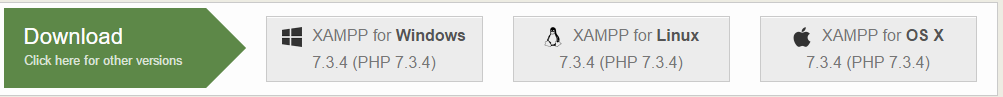
\includegraphics[scale=0.5]{figures/xampp}
\caption{Versi Terbaru XAMPP}
\end{figure}

File xampp-windows-x64-7.3.4-0-VC15-installer berukuran cukup besar, sekitar 149MB. Simpanlah file ini dimana kita inginkan.
Setelah file XAMPP sudah di download, kita akan menginstallnya dengan cara double klik pada aplikasi tersebut dan akan mucul peringatan sebagai berikut.

 \begin{figure}[h]
\centering
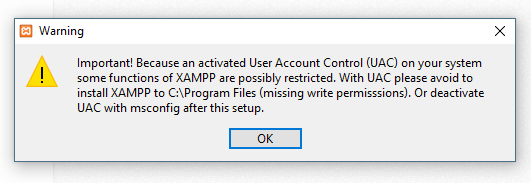
\includegraphics[scale=0.5]{figures/uac}
\caption{User Account Control}
\end{figure}

Peringatan ini berkaitan dengan keamanan pada versi Windows Vista keatas dan jika XAMPP akan di install pada folder C mungkin akan terjadi pembatasan hak akses terhadap XAMPP yang berjalan tidak normal. Silahkan klik tombol OK untuk melanjutkan install maka akan muncul jendela awal install. Silahkan klik next.

 \begin{figure}[h]
\centering
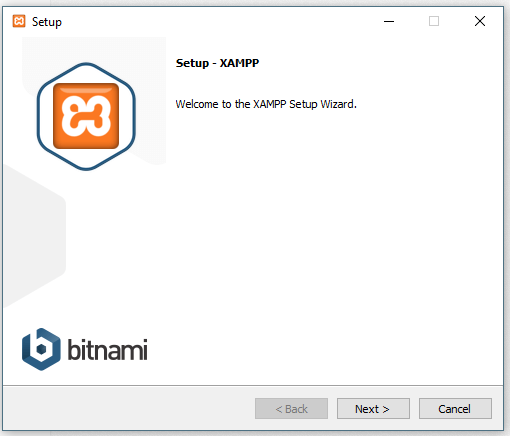
\includegraphics[scale=0.5]{figures/jendelaawal}
\caption{Jendela Awal}
\end{figure}

Jendela selanjutnya adalah Select Component. Dalam jendela ini kita dapat memilih modul atau aplikasi apa saja yang akan kita install. Dalam tahap ini kita akan menceklis semua pilihan selanjutnya klik next untuk melanjutkan.

\begin{figure}[h]
\centering
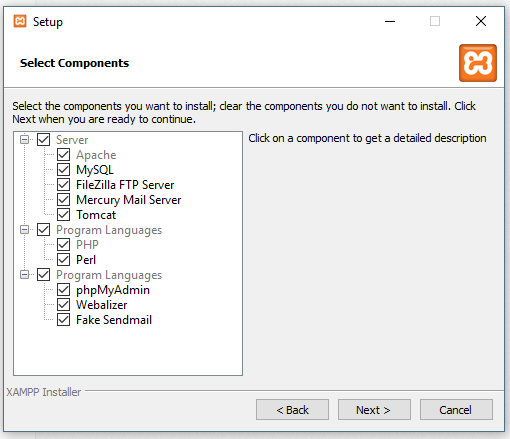
\includegraphics[scale=0.5]{figures/selectcomponent}
\caption{Select Component}
\end{figure}

Jendela selanjutnya adalah Installation Folder. Dalam jendela ini kita dapat mengubah lokasi dimana kita akan menyimpan file-file XAMPP. Sebagai contoh kita akan menyimpan file XAMPP di drive E dengan nama folder xampp agar mudah di ingat. Untuk melanjutkan klik next.

\begin{figure}[h]
\centering
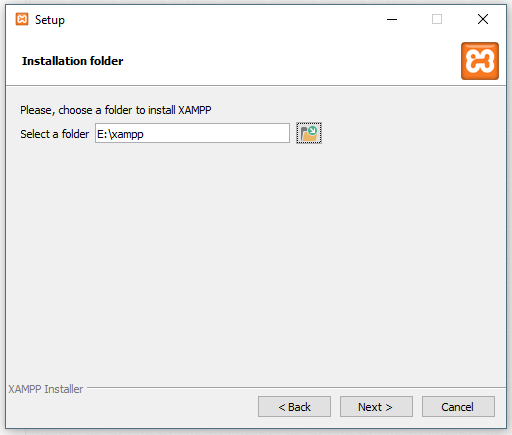
\includegraphics[scale=0.5]{figures/installationfolder}
\caption{Installation Folder}
\end{figure}

Jendela berikutnya adalah Bitnami for XAMPP. Dalam hal ini XAMPP menawarkan Bitnami sebagai cara cepat untuk install CMS seperti wordpress, drupal, dan joomla. Kemudian klik next.

\begin{figure}[h]
\centering
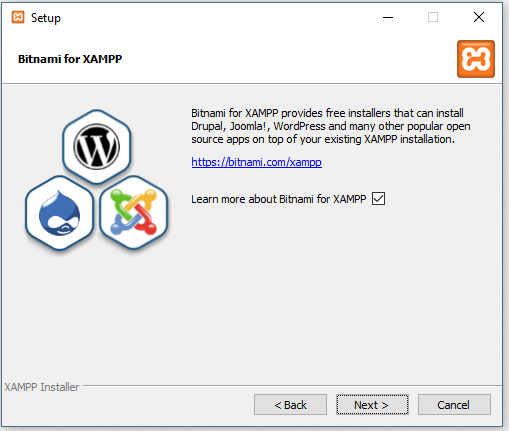
\includegraphics[scale=0.5]{figures/bitnamiforxampp}
\caption{Bitnami for XAMPP}
\end{figure}

Jendela berikutnya adalah pemberitahuan bahwa kita siap untuk menginstall XAMPP, Klik next dan XAMPP akan memulai  proses penginstallan.

\begin{figure}[h]
\centering
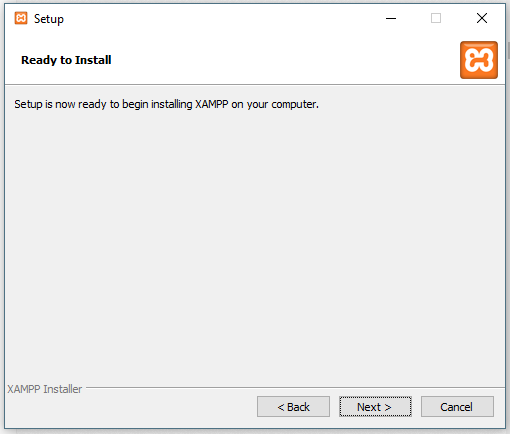
\includegraphics[scale=0.5]{figures/readytoinstall}
\caption{Ready to Install}
\end{figure}

\begin{figure}[h]
\centering
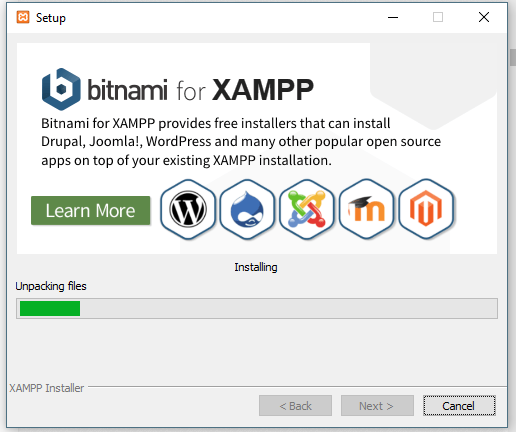
\includegraphics[scale=0.5]{figures/setup}
\caption{Proses Penginstallan}
\end{figure}

Setelah proses penginstallan hampir selesai akan muncul jendela Windows Security Alert pada gambar 5.9 karena Windows Defender Firewall mendenteksi Apache HTTP Server. Untuk lanjut klik Allow access.

\begin{figure}[h]
\centering
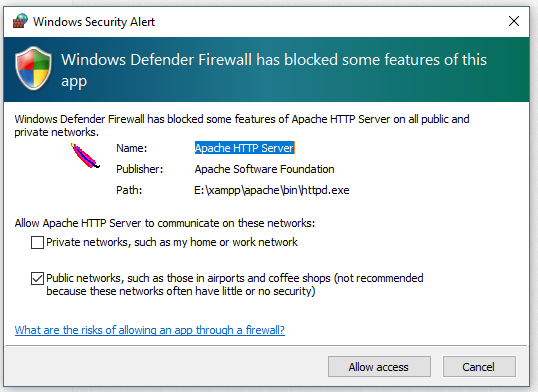
\includegraphics[scale=0.5]{figures/windowssecurityalert}
\caption{Windows Security Alert}
\end{figure}

Proses penginstallan XAMPP sudah selesai pada gambar 5.10 maka akan muncul jendela Completing, dalam bagian ini kita dapat memilih untuk langsung menggunakan XAMPP atau tidak. Jika ingin langsung memakai, ceklis pada Do you want to start the Control Panel now? lalu klik finish. Jika tidak maka hilangkan ceklis dari  Do you want to start the Control Panel now? lalu klik finish.

\begin{figure}[h]
\centering
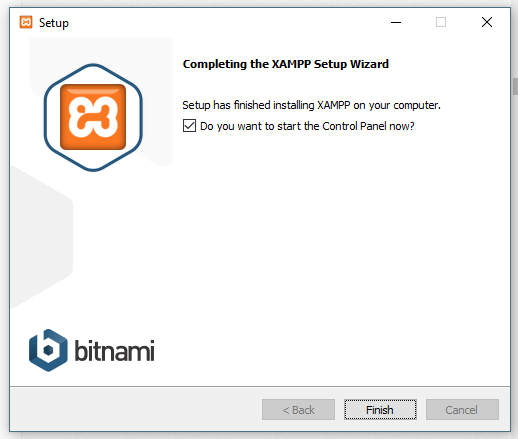
\includegraphics[scale=0.5]{figures/selesaiinstall}
\caption{Selesai Install}
\end{figure}

\subsection{Menguji Instalasi XAMPP}
Sesuai dengan namanya, jendela XAMPP Control Panel adalah jendela yang digunakan untuk mengontrol apa saja modul atau aplikasi apa saja yang ingin kita jalankan. Jika ingin membuka manual maka kita dapat membuka dengan cara dari menu Start->All Programs->XAMPP->XAMPP Control Panel. Untuk menguji instalan XAMPP ini, silahkan klik tombol Start pada modul apache dan MySQL. Jika tidak ada masalah maka akan tampil warna hijau pada bagian modul ini.

\begin{figure}[h]
\centering
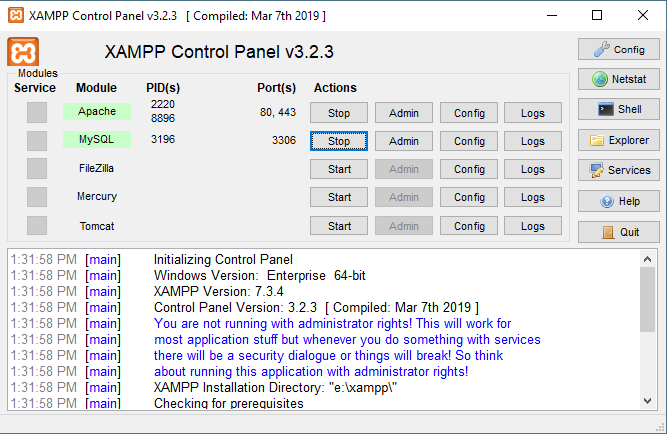
\includegraphics[scale=0.5]{figures/controlpanel}
\caption{XAMPP Control Panel}
\end{figure}

Selanjutnya buka web browser dan ketikan localhost pada address bar kemudian enter maka akan muncul dengan otomatis localhost/dashboard semuanya telah terinstall dengan baik.

\begin{figure}[h]
\centering
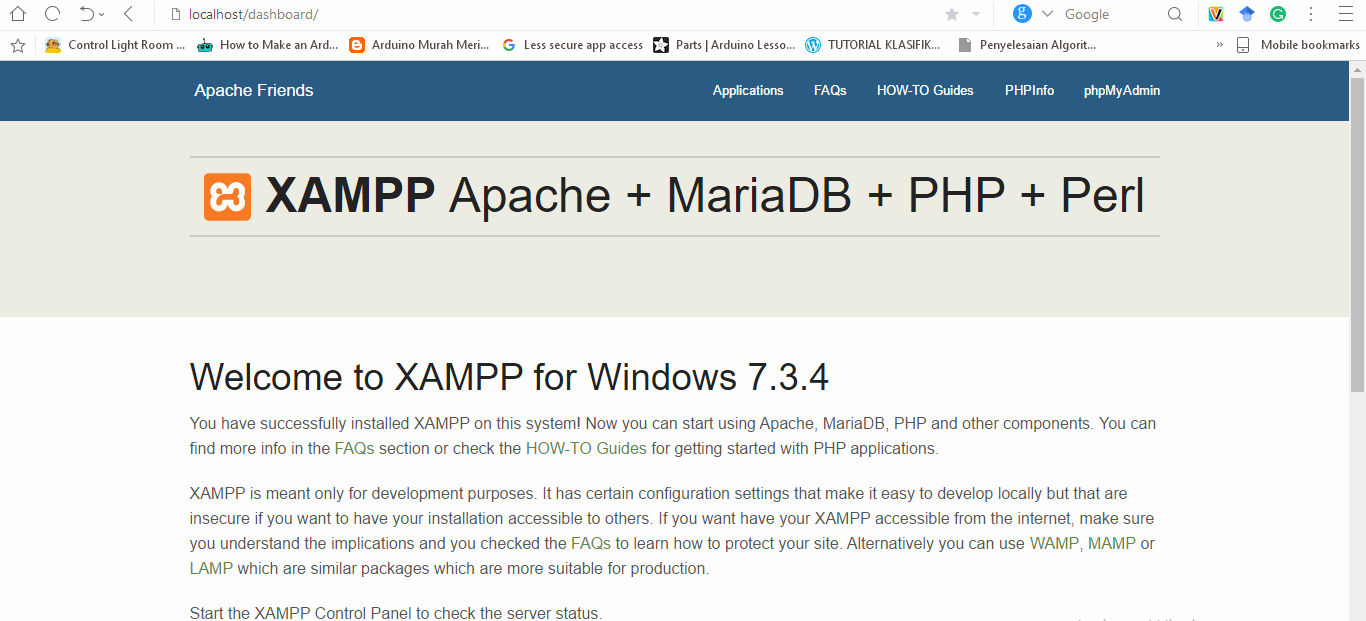
\includegraphics[scale=0.3]{figures/dashboard}
\caption{Localhost Dashboard}
\end{figure}

Jika ingin melihat versi PHP kita secara mendalam silahkan klik PHPInfo di pojok kanan atas. Disini kita dapat melihat bahwa PHP yang kita pakai sudah versi 7.3.4.

\begin{figure}[h]
\centering
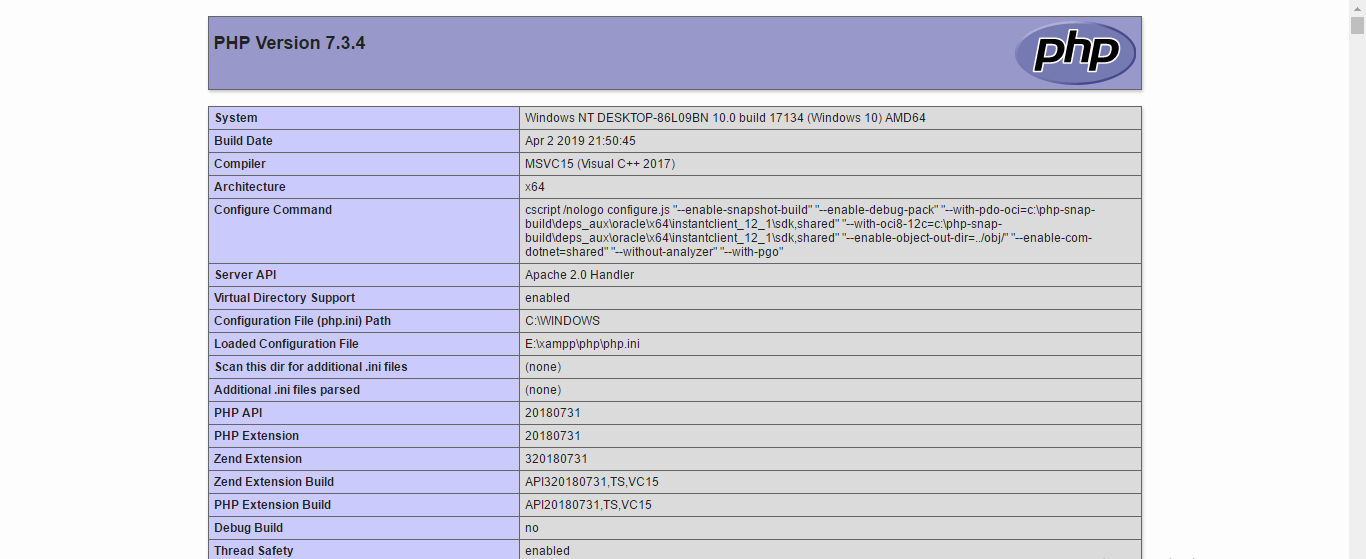
\includegraphics[scale=0.4]{figures/versiphp}
\caption{Versi PHP}
\end{figure}


\section{Localhost}
Localhost adalah server lokal atau sebuah web server yang bekerja pada laptop anda. Alamat IP dari localhost adalah 127.0.0.1.
Jadi localhost terletak pada laptop anda. Anda membutuhkan localhost itu sendiri untuk menjalankan file .php yang telah di jelaskan sebelumnya di pengenalan php. PHP hanya dapat berjalan pada sisi sever dan karenanya PHP disebut sebagai pemrograman server side atau pada sisi server.
\par
Localhost dijadikan server pada saar pengembangan aplikasi yang berbasis web sebelum di hostingkan. Localhost hanya dapat diakses laptop pada browser anda dengan alamat http://127.0.0.1 atau http://localhost. Maka halaman akan ditampillkan ke localhost projek aplikasi yang sedang anda buat. 
